\subsection{Materials List}
The following materials were used to design, assemble, and test the AFER systems: Arduino controller (1), USB Cable (1), CAT 6e Cable (1), a computer with the capability to run Arduino Integrated Development Environment (IDE), Autodesk Fusion 360 Computer Aided Design(CAD) software and Open Source Fritzing Hardware Prototyping Software, a servomotor with $360^{\circ}$ rotation (1), High-torque servomotor with $180^{\circ}$ rotation (1), Servomotor horn – 4 prong (1), servo horn 2-prong (1), 30 row bread board (1), composite dowel (1) , 3-D printed Polylactic Acid (PLA) \textit{l1}, 3-D printed PLA dowel mount (1), 3-D printed PLA servomotor mounts (2), plywood base (1), wood clamps (2), Cat Toys – Feather (1) / Mouse (1), C-Clamp (2), Bosch 12v Lithium Ion Battery Power Drill (1), IRWIN 15 Piece Drill bit set – sizes $\frac{1}{16}$ to $\frac{3}{8} (1)$, String (1), Bolts (10), Superglue (1), Sewing ruler (1), Tape measure (1), 3-D printer – Monoprice Maker Select v2, PLA filament, etc. 

\subsection{Methods}
The following high-level steps were used:
\begin{itemize}
\item Step 1: Design and build the system
\item Step 2: Solve the kinematics and Jacobian
\item Step 3: Develop and implement movement patterns
\item Step 4: Experimental evaluation of the design
\item Step 5: Performance Analysis
\end{itemize}

\subsubsection {Designing the Robot}
The first step in designing the robot was to hand sketch the initial block diagram design for AFER v1 and v2. The hand sketches were then converted to basic diagrams on a computer, shown in Fig.1 below:

\begin{figure}[h!]
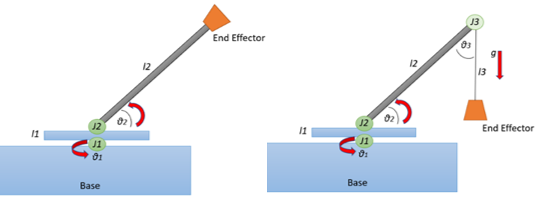
\includegraphics[width=\columnwidth]{Fig1.png}
\caption{AFER v1 and v2 sketches.}
\label{1}
\end{figure}


For both AFER versions: J1 is the first joint, J2 the second joint,  \textit{l1} the height of the rotating platform between J1 and J2,  \textit{l2} the length of the actuated arm, $\theta_{1}$ the angle of rotation about the z-axis, and $\theta_{2}$ the angle of \textit{l2} with respect to the x-axis. AFER v2 has three additional parameters: J3 as joint 3, \textit{l3} as the length of the string attached to J3, and $\theta_{3}$ as the angle between \textit{l2} and \textit{l3}.
Once the overall design was determined, the pieces requiring CAD rendering - \textit{l1}, servomotor mount 1 (SM1), servomotor mount 2 (SM2), and the dowel mount (DM) – were sketched by hand. Once sketched, measurements of the servomotors and dowel were taken using a sewing ruler and tape measure. Those measurements were then used to inform the exact size and shape of the part builds. The Autodesk Fusion 360 software was used to build and render each of the parts. Fig.2 shows the CAD rendering and completed print of the SM1 piece, as an example.

\begin{figure}[h!]
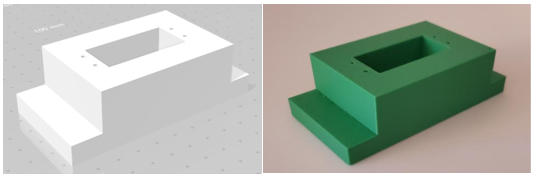
\includegraphics[width=\columnwidth]{Fig2.png}
\caption{AFER SM 1 CAD rendering (left) and printed piece (right).}
\label{2}
\end{figure}

\subsubsection{Building the Robot}
When designing the pieces to be 3-D printed, there were sets of bolt holes that were not rendered in CAD to allow greater flexibility while assembling and to allow for adjustments to ensure proper alignment of the axes. The necessary holes for those bolts were measured and drilled individually during the assembly process. The robot was built beginning with the topmost piece and working down to the base to simplify the process of establishing the z-axis for joints 1 and 2 as coincident. 
On the front plate, a hole was drilled at a height that would ensure the center axis of the dowel would intersect orthogonally with the rotational axis of J2, and the servomotor horns were screwed into DM. Servo Mount 2 (SM2) was then mounted to the side of \textit{l1}, positioning J2 directly above J1 to avoid altering the z axis. A wiring port and inset bolt holes were also drilled into SM2. A similar process was used on \textit{l1}.
The high torque servomotor was then fitted into SM2 and attached using the printed bolt holes; once secured to the mount, the servo was connected to DM. Subsequently, the $360^{\circ}$rotation servomotor was fitted and bolted into the mount. Mounting the 4-prong servomotor horn to \textit{l1} was accomplished using super glue and screws. The SM2, DM, \textit{l1} configuration was placed onto the servomotor in SM1 once the glue had dried. 
The final build step was to attach the AFER robot to the plywood base. The same 3-D printed core parts were used for both v1 and v2; to switch between versions, the directly connected end effector was replaced with a string and the end effectors were then attached to the string. Fig.3 shows the fully assembled AFER v1 and v2.

\begin{figure}[h!]
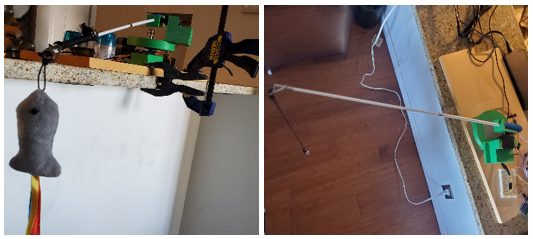
\includegraphics[width=\columnwidth]{Fig3.png}
\caption{Fully assembled AFER v1 (left) and v2 (right).}
\label{3}
\end{figure}

Wiring for the Arduino and two servomotors was accomplished by stripping the CAT 6e cable and using the interior wires to connect between Arduino ports, the bread board, and the positive, negative and control wires for both servomotors. To ensure adequate power for running multiple servomotors, the bread board was connected to an external 5v power source. Fig.4 is a wiring diagram built using an open source wiring tool called Fritzing to illustrate the connections needed to power and control the AFER core configuration and subsequently, AFER v1 and v2.

\begin{figure}[h!]
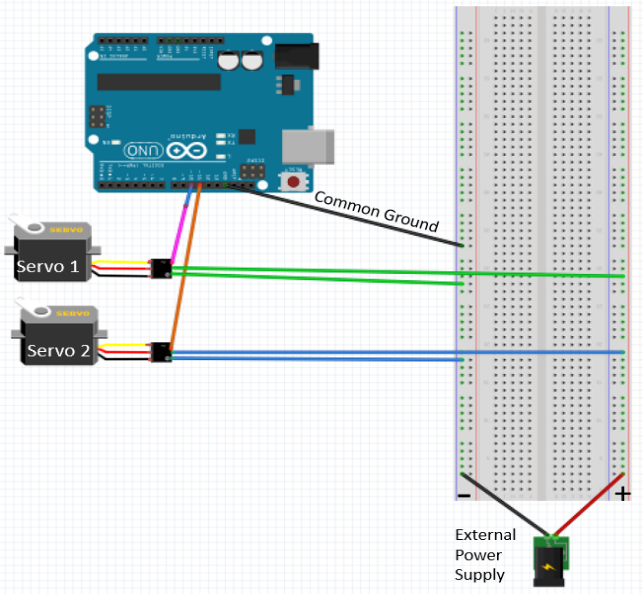
\includegraphics[width=\columnwidth]{Fig4.png}
\caption{AFER Circuit Diagram.}
\label{4}
\end{figure}

\subsubsection{Solving the Kinematics and Jacobian}
The process for solving the kinematics is described in greater depth in Section V. The process for deriving the Jacobian for AFER v1 and v2 is described in Section VI.

\subsubsection{Developing and Implementing Movement Patterns}
The movement patterns selected were a simple back-and-forth oscillation, an up-and-down oscillation, and a combination of both types of oscillation. Position control was used for all three movement patterns. 
The Arduino Servo Library contains a function “Sweep” which swings the shaft of the servomotor back and forth across a $180^{\circ}$ arc. The source code for this function was used as a starting point for both the up-and-down and back-and-forth oscillation patterns \cite{Arduino2020sweep}. Each oscillation pattern was comprised of two loops, one to sweep the servo from 0 to the maximum angle - $45^{\circ}$ for servo 2 and $180^{\circ}$ for servo 1 – and a second loop to sweep the servo from the maximum angle back to 0. The combination of both oscillation patterns was achieved by combining the four loops from the previous code into two loops that actuated both servos simultaneously.
All three of those motion patterns were simplistic and did not require any complex path planning or trajectory generation to implement. To avoid erratic robot behavior during initial testing, the robot pieces were separated, and the code was tested on the servomotors with no load. The initial testing involved sweeping servo 1 in a $90^{\circ}$ arc and servo 2 in a $45^{\circ}$ arc; the testing with those parameters was successful.
The code was then tested on the full common core unit. Upon initial assembly and motion testing, the servo horn and motor at J1 continuously became disconnected after 2-3 oscillations. To add stability, the horn and motor were superglued together. Once the glue dried, J1 was significantly more stable and able to withstand the necessary continuous oscillation. 
Once AFER was securely assembled, it became clear that $180^{\circ}$ was too large of an angle for servo 1 when accounting for the full length of \textit{l1} and space in which the kittens could play; the sweep angle for servo 1 was, therefore, reduced to $90^{\circ}$. Additionally, to resolve an increment error, the servo 1 code was updated to increment by 2 rather than 1. 

\subsubsection{Test Subjects}
The robot was tested on two kittens – one male, one female – each approximately six months old. The female kitten, named Klunk, was solid black; she weighed 6.1lbs at the time of testing. Her demeanor was timid and easily startled. The male kitten, named Traximus, was black with white tuxedo markings; he weighed 6.4lbs at the time of testing, and his demeanor was outgoing and curious.

\subsubsection{ Experimentation and Testing (Evaluation) }
Once fully assembled, the robot was tested to ensure that it could be operated effectively and safely prior to the introduction of the test subjects. The experimentation and test procedures are documented in greater depth in Section VII.

\subsubsection{Safety Considerations}
The robot was designed with the following safety considerations: 
\begin{itemize}
\item The Servomotors selected do not create adequate force to cause damage to the kittens.
\item The dowel selected was made of partially compliant material that was unlikely to cause injury if it collided with the one of the kittens.
\item Trajectories that simulated a wrapping movement were avoided to minimize the likelihood of accidentally tangling the kittens in the AFER v2 string.
\item For AFER v1, the robot was placed on a box and secured with C clamps to prevent it from falling.
\item For AFER v2, a set of C clamps were used to secure the robot base to a table and ensure the kittens could not pull the robot onto themselves during play and cause injury.
\item The wires used to connect the robot and laptop were covered with cardboard or paper as much as possible to prevent the kittens from chewing the wires as well as protect from accidental shocks.
\end{itemize}

\subsubsection{Performance Analysis}
Performance of the robot was ascertained predominately by visually observing the behavior of the system and the test subject’s reactions to it. Some servo data was observed in the Arduino Serial Monitor to verify the system movement patterns were implemented properly. See Section VII for further details.

\subsection{Assumptions}
The design and modeling assumptions are below:
\begin{itemize}
\item The encoders in the servomotors had sufficient precision for this task
\item For v1, all linkages were modeled as rigid linkages 
\item For v2, J3 was modeled as a passive joint that was frictionless, had no damping, and had no elasticity
\item For v2, the link between J3 and the end effector was assumed to be rigid
\item For both robots, when solving the kinematics, static stability would be assumed at all points
\end{itemize}